\chapter{FUS mutant mice show progressive changes in mitochondrial and ribosomal transcripts}

\label{chapter:fus_mouse}

Work presented in this chapter has been published as part of \citep{Devoy2017}. See appendices for full reproduction of the published manuscript.

\section{Overview}
This chapter describes work carried out in collaboration with Dr Anny Devoy of the UCL Institute of Neurology. 
Dr Devoy created a "humanised" mouse model of ALS resulting from a mutation in the FUS RNA-binding protein. 
I analysed RNA-seq taken from two tissues and time points and demonstrated a specific transcriptomic signature that correlates with a progressive neurodegenerative phenotype seen in aged mutant mice.
This involves the downregulation of mitochondrial and ribosomal transcripts.

\section{Contributions}
\begin{itemize}
	% Check with Pietro
	\item Transgenic mice were created by Dr Anny Devoy
	\item RNA sequencing libraries were prepared by Dr Anny Devoy
	\item RT-PCR validation was performed by Dr Anny Devoy
	\item Fig. \ref{fig:delta14_structure} was created by Dr Anny Devoy
\end{itemize}
All bioinformatic analysis and interpretation was designed and performed by myself in consultation with Dr Anny Devoy and my supervisors. 


\section{Background}
% REWRITE
All previous studies alter FUS expression to levels that wildly differ to the normal biological situation. Overexpression or knockout are clearly toxic but these do not help to differentiate the effects of the mutations of normal FUS function. 
%recently
Until recently there have been no studies where the effects of a human FUS mutation are seen on the mouse at a physiological level of expression. 
The FUS $\Delta$14 mutation was found in an early onset ALS patient who died at the age of 22 following a very rapid disease course \citep{DeJesus-Hernandez2010}. The mutation alters the 3\'\ splice site of exon 14 of FUS, causing it to be skipped.  Comparison of the $\Delta$14 mutation with other, late-onset ALS causing mutations have shown an increased propensity by FUS $\Delta$14 to accumulate in the cytoplasm \citep{Verbeeck2012}. Analysis of mice carrying a single copy of the FUS $\Delta$14 mutation enables a reconstruction of progressive neurodegenerative disease. By analysing RNA-seq data collected across the lifespan of the mice, I can observe specific RNA dysregulation caused by the mutant protein.

\subsection{The FUS $\Delta$14 mouse is a humanised model of ALS}
The FUS $\Delta$14 mouse was created by directed mutagenesis of the mouse Fus exon 14 splice site as well as humanisation of exon 15 with 4 separate mutations.The result of splicing exons 13 and 15 together is a frameshift which at the protein level removes the C-terminal nuclear localisation signal (Fig. \ref{fig:delta14_structure}A) but leaves a novel peptide sequence which can used to create specific antibodies. Reverse-transcription PCR to detect FUS mRNA showed the $\Delta$14 FUS mRNA to be expressed at a similar level to wildtype FUS (Fig. \ref{fig:delta14_structure}B). 


\begin{figure}[h!]
	\begin{center}
		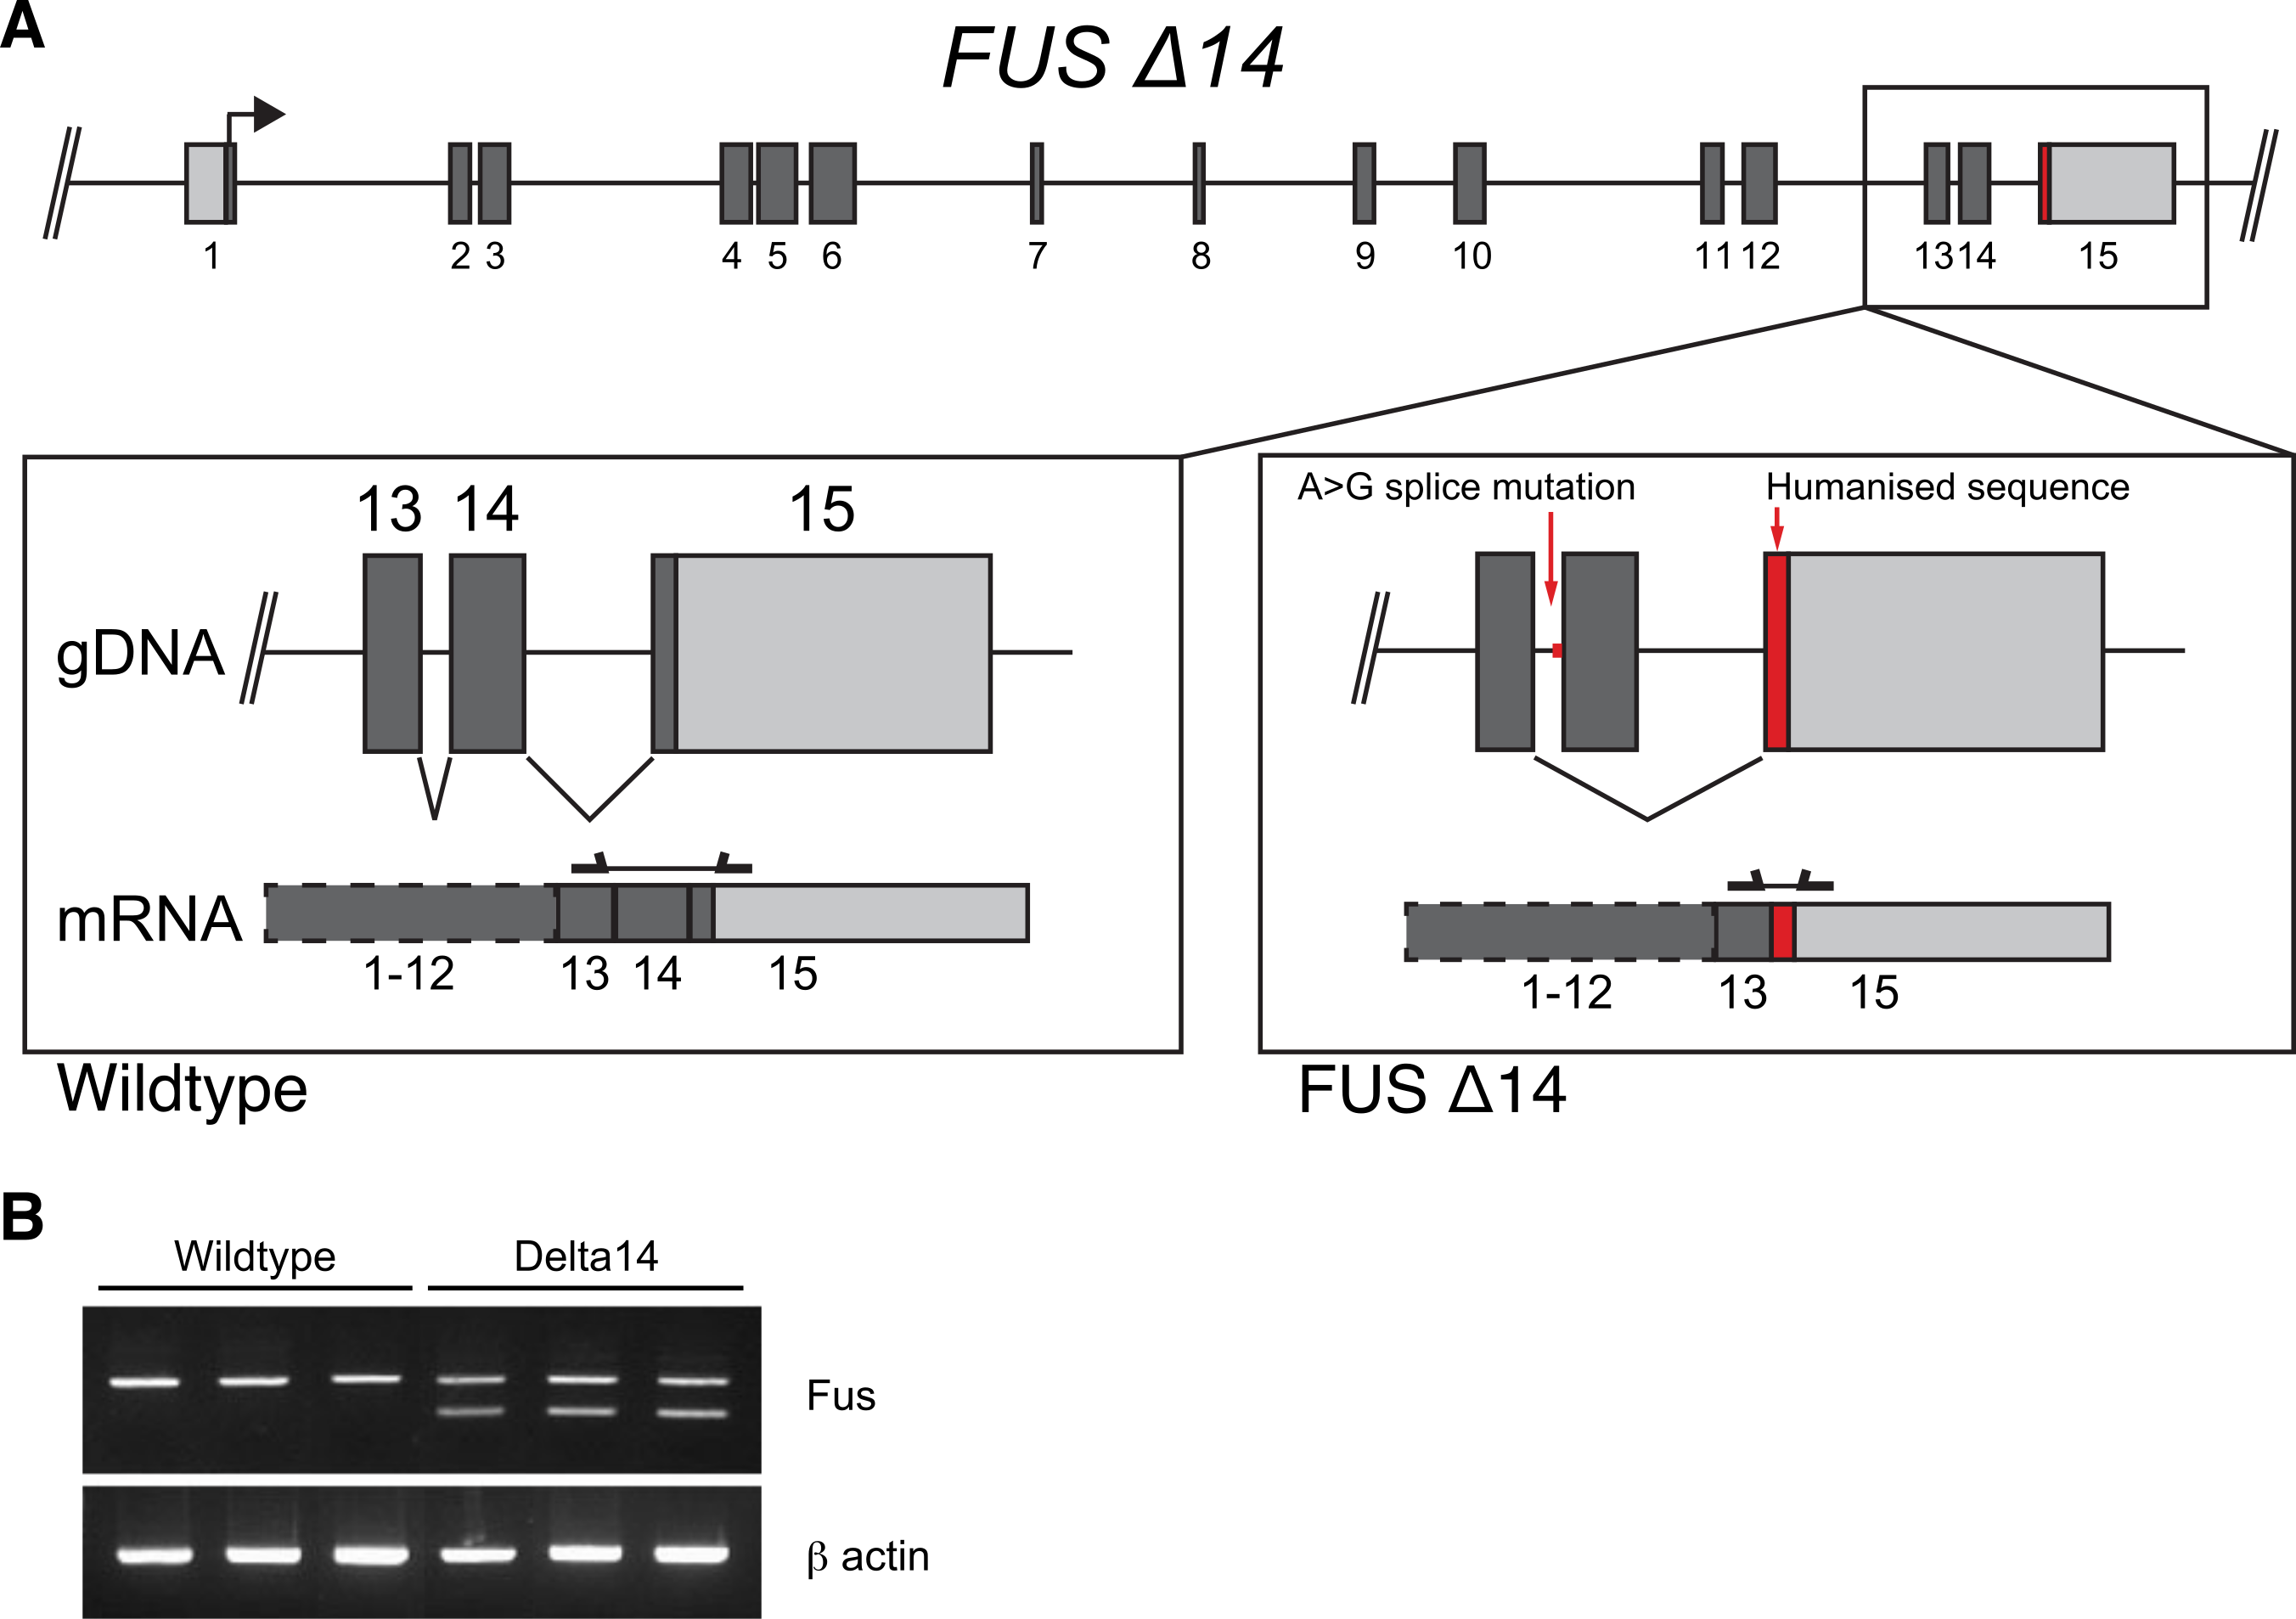
\includegraphics[width=\textwidth]{Figures/04_fus_mice/anny_FUS_schematic.png}
	\end{center}
	\caption[The FUS $\Delta$14 model]{
		\textbf{The FUS $\Delta$14 model.}
		\textbf{(A)} The FUS locus with a closeup of the terminal three exons in the wildtype mouse (left) and the FUS $\Delta$14 mouse (right). 
		\textbf{(B)} RT-PCR of FUS mRNA from spinal cord of wildtype and mutant mice.
	}
		\label{fig:delta14_structure}
\end{figure}


\section{Methods}

\subsection{Data preparation}
All RNA-seq data used is listed in table \ref{table:fus_mice_rnaseq}. All samples were aligned to the mm10 mouse reference genome using the previously discussed analysis pipeline.


\begin{table}[h!]
	\caption[All RNA-sequencing data used in this study]{
		\textbf{All RNA-sequencing data used in this study}
	Library info describes the type of library prepared, the length of each read and whether the sequencing was single or paired end. PE: paired end sequencing. Depth is defined the number of uniquely mapped read pairs, in millions.
}
	\label{table:fus_mice_rnaseq}
	\begin{center}
		\begin{small}
			\begin{tabular}{llllp{1.5cm}llll}
				Species & Cell type & Time point & Library info & Depth & Number\\
				\hline
				Mouse & Spinal Cord & 3 months & stranded mRNA 75bp PE & 33-43M & 4 vs 4\\
				Mouse & Spinal Cord & 12 months & stranded mRNA 75bp PE & 35-46M & 4 vs 4\\ 
				Mouse & Motor/Frontal Cortex & 3 months & stranded mRNA 75bp PE & 35-52M & 4 vs 4\\
				Mouse & Motor/Frontal Cortex & 12 months & stranded mRNA 75bp PE & 35-48M & 4 vs 4\\ 
			\end{tabular}
		\end{small}
	\end{center}
\end{table}

\subsection{Differential gene expression}
Differential expression was carried out with \textit{DESeq2} \citep{Love2014} comparing wildtype with mutant mice. All P-values were adjusted at a false discovery rate of 10\%. To assess the variance between each sample the raw counts for each gene were normalised to account for library size and then normalised again by the regularized log normalisation method \citep{Love2014}. The counts were further transformed into Z-scores, which express the number of standard deviations from the mean of all counts for that gene. Heatmaps were created for all significantly differentially expressed genes using the \textit{pheatmap} R package \citep{Kolde2012}.  

\subsection{Gene Ontology analysis}
Gene ontology (GO) analysis is a method to extract inference from gene expression experiments by annotating each gene and protein within a unified vocabulary of molecular and cellular function. This can be used to identify dyregulated pathways or broader trends \citep{Ashburner2000}. For each differential expression results set the multiple correction threshold was dropped to P < 0.005 for each gene to increase the number of input genes. The resulting list of hits was then annotated for GO terms and a hypergeometric test was applied to test the enrichment of particular categories against a background set of genes. It is important to account for selection bias for long genes in RNA-seq data as longer genes have more power to be differentially expressed than shorter genes \citep{Young2010}. The R package \textit{GOseq} implements a GO term annotation and enrichment test which takes account of this length bias \citep{Young2010}. The resulting P-values were then Bonferroni corrected for multiple testing. In each category the number of genes that were up- or downregulated in the $\Delta$14 mice relative to wildtype littermates were expressed as a percentage. 

\subsection{Differential splicing}
Differential splicing was analysed for the 12 month spinal cord samples using SGSeq \citep{Goldstein2016} to find novel and annotated splicing events. Counts of inclusion and exclusion were used to fit a model with DEXSeq \citep{Anders2012} to test the effect of condition on splicing event inclusion. Splicing events were reported at FDR < 0.05.

\section{Results}

\subsection{Gene expression changes are tissue- and time point-specific}

\begin{figure}[h!]
	\centering
	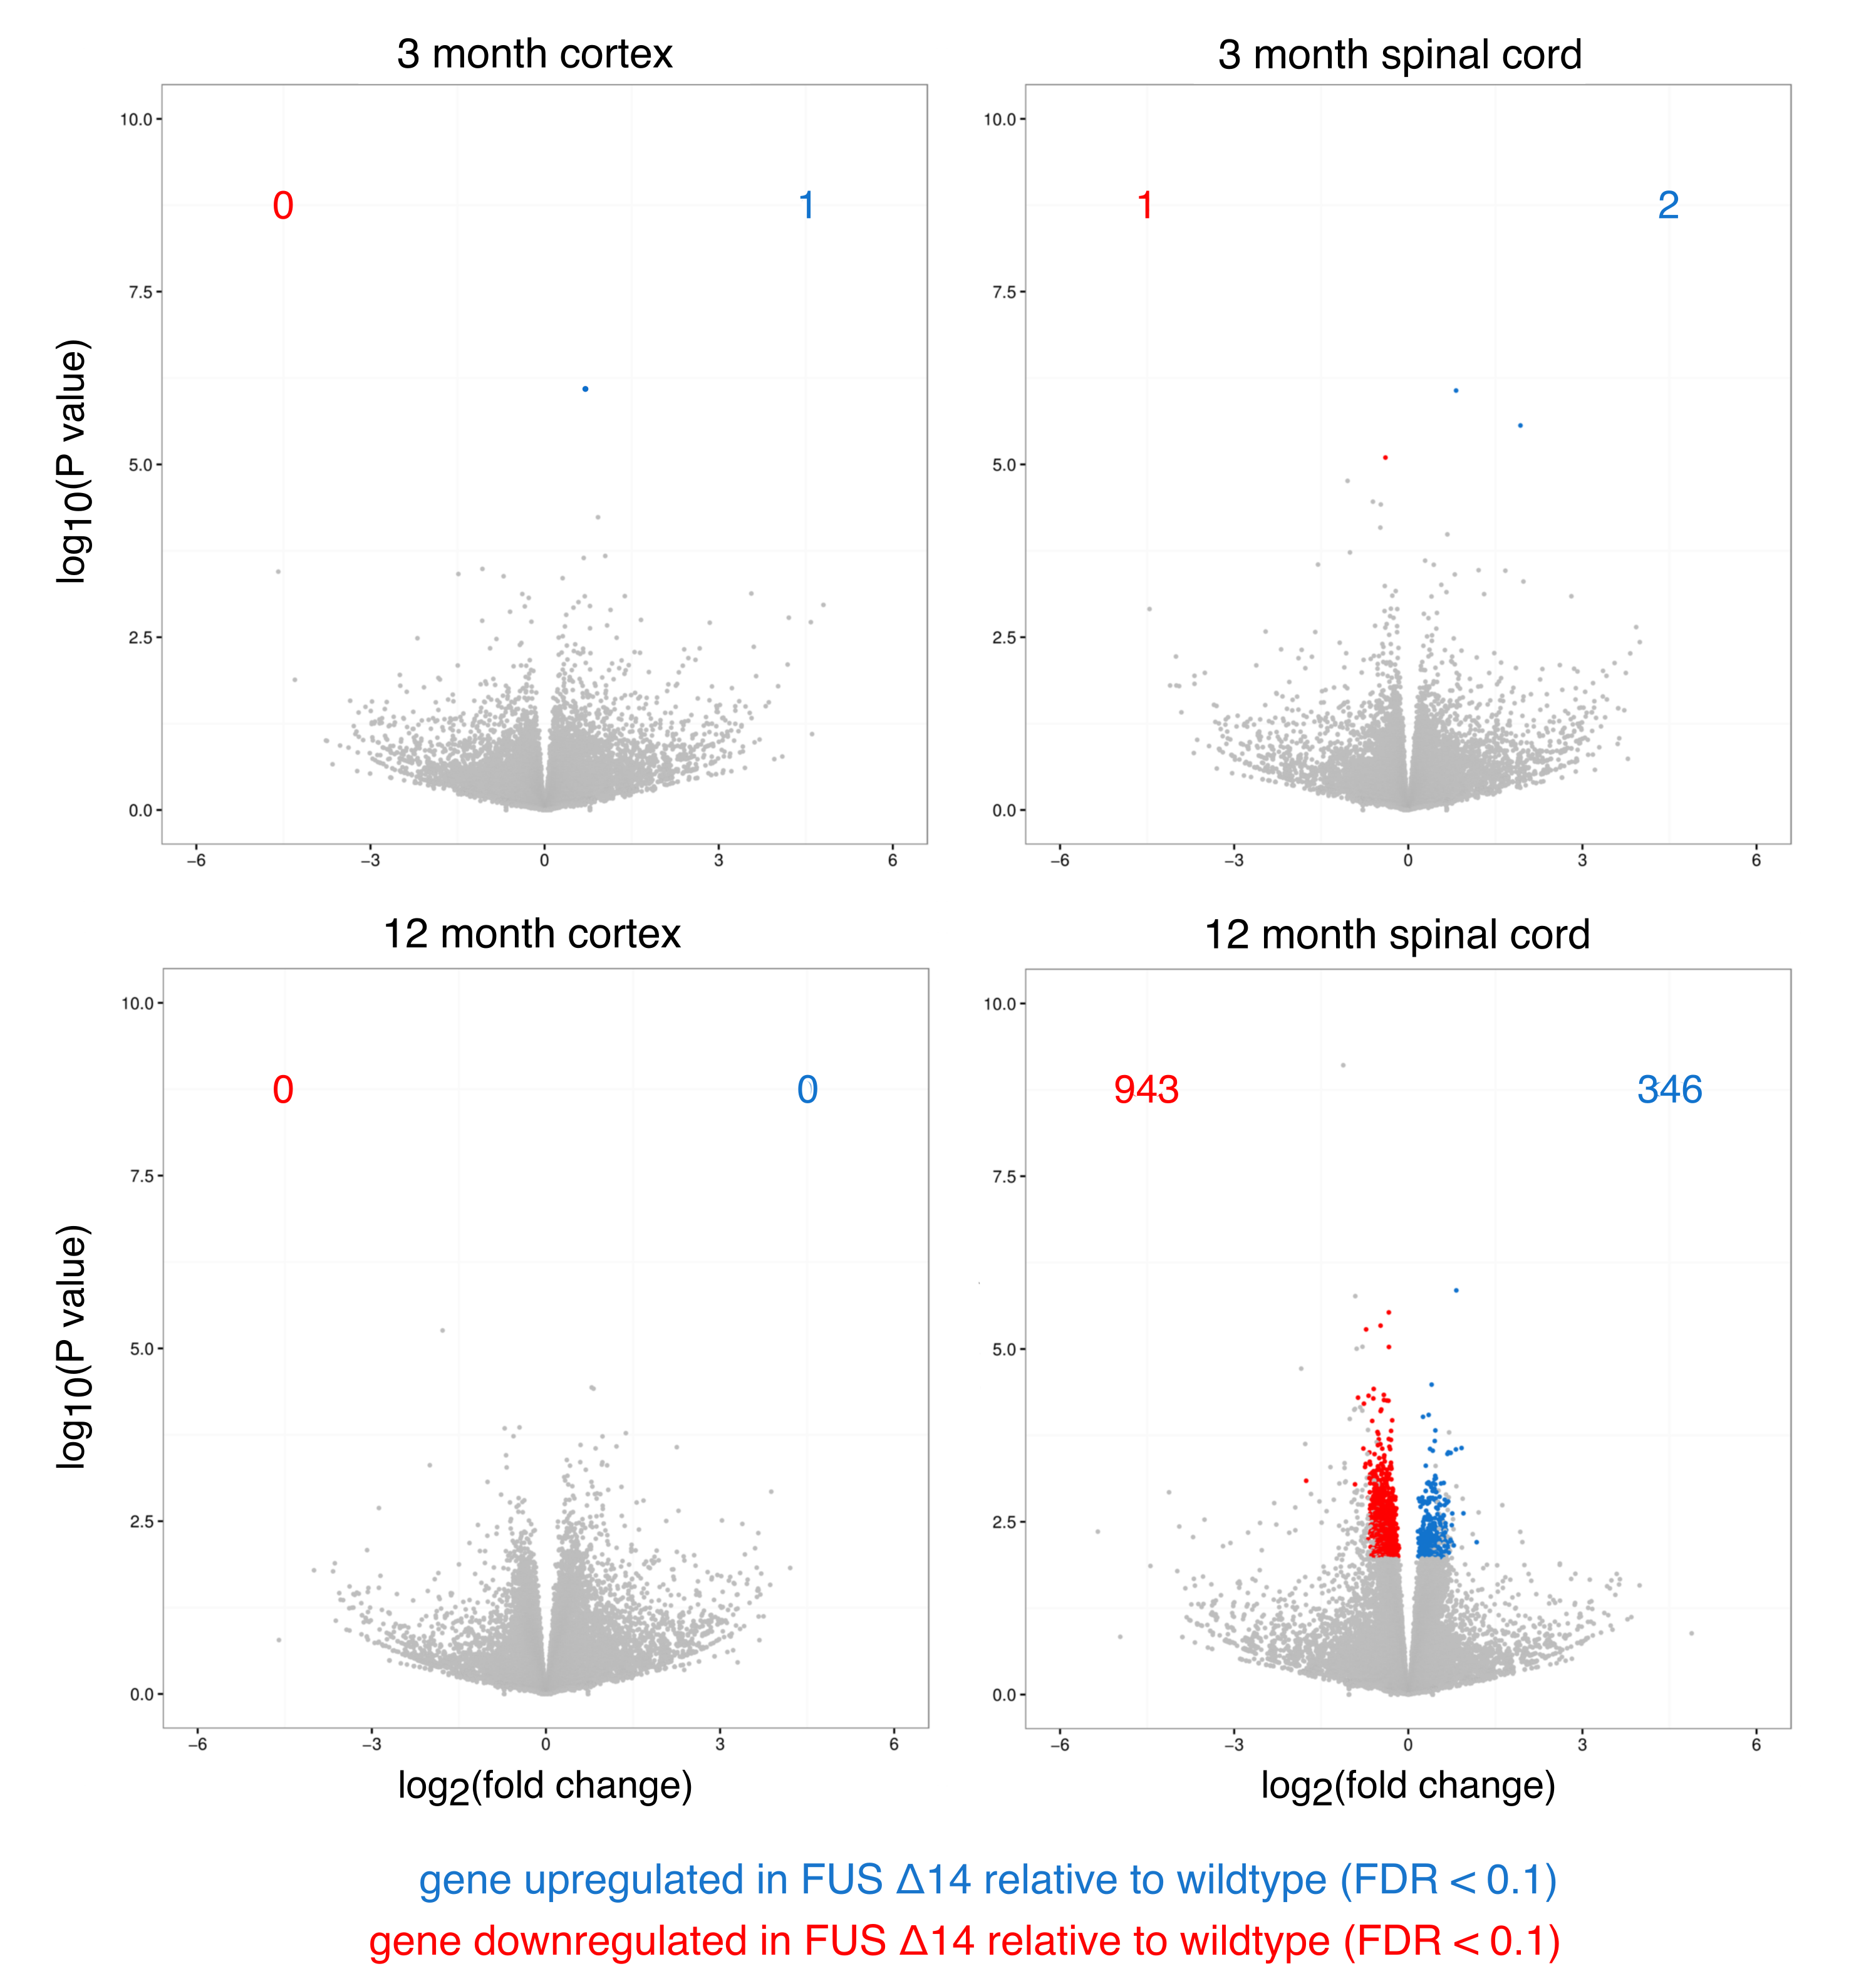
\includegraphics[width=\textwidth]{Figures/04_fus_mice/anny_volcanos.png}
	\caption[Differential gene expression analysis on the $\Delta$14 mouse]{
		\textbf{Differential gene expression analysis on the $\Delta$14 mouse across two tissues and time points.}
		Each gene is represented as a point. The x axis is the $log_2$ of the ratio between the average expression in the $\Delta$14 mice against that of the wildtype mice. The y axis is the $log_10$ of the unadjusted P-value for the differential expression test. The numbers of upregulated genes (adjusted \textit{P} < 0.1 with a $log_2$(fold change) > 0) are in blue and the the downregulated ( adjusted \textit{P} < 0.1 with $log_2$(fold change) < 0) are in red.
	}
	\label{fig:delta14_volcanos}
\end{figure}

To examine progressive changes in RNA regulation, total RNA was extracted from both spinal cord and forebrain from mice across two time-points: 3 months and 12 months. Four male mice of each genotype ($\Delta$14 and wildtype littermate) were used at each timepoint. At 3 months of age, the forebrain and spinal cord samples had 1 and 3 genes differentially expressed respectively. At 12 months of age there were no differentially expressed genes found in the forebrain but 1,289 found in the spinal cord, with genes predominantly decreased in expression (Fig. \ref{fig:delta14_volcanos}). To examine the variance between each sample in the 12 month spinal cord dataset, the read counts for each gene were normalised and converted to Z-score values. Plotted as a heatmap it is clear that the size of each change is small and there is considerable inter-condition variability (Fig. \ref{fig:delta14_heatmap}).


\begin{figure}[h!]
	\centering
	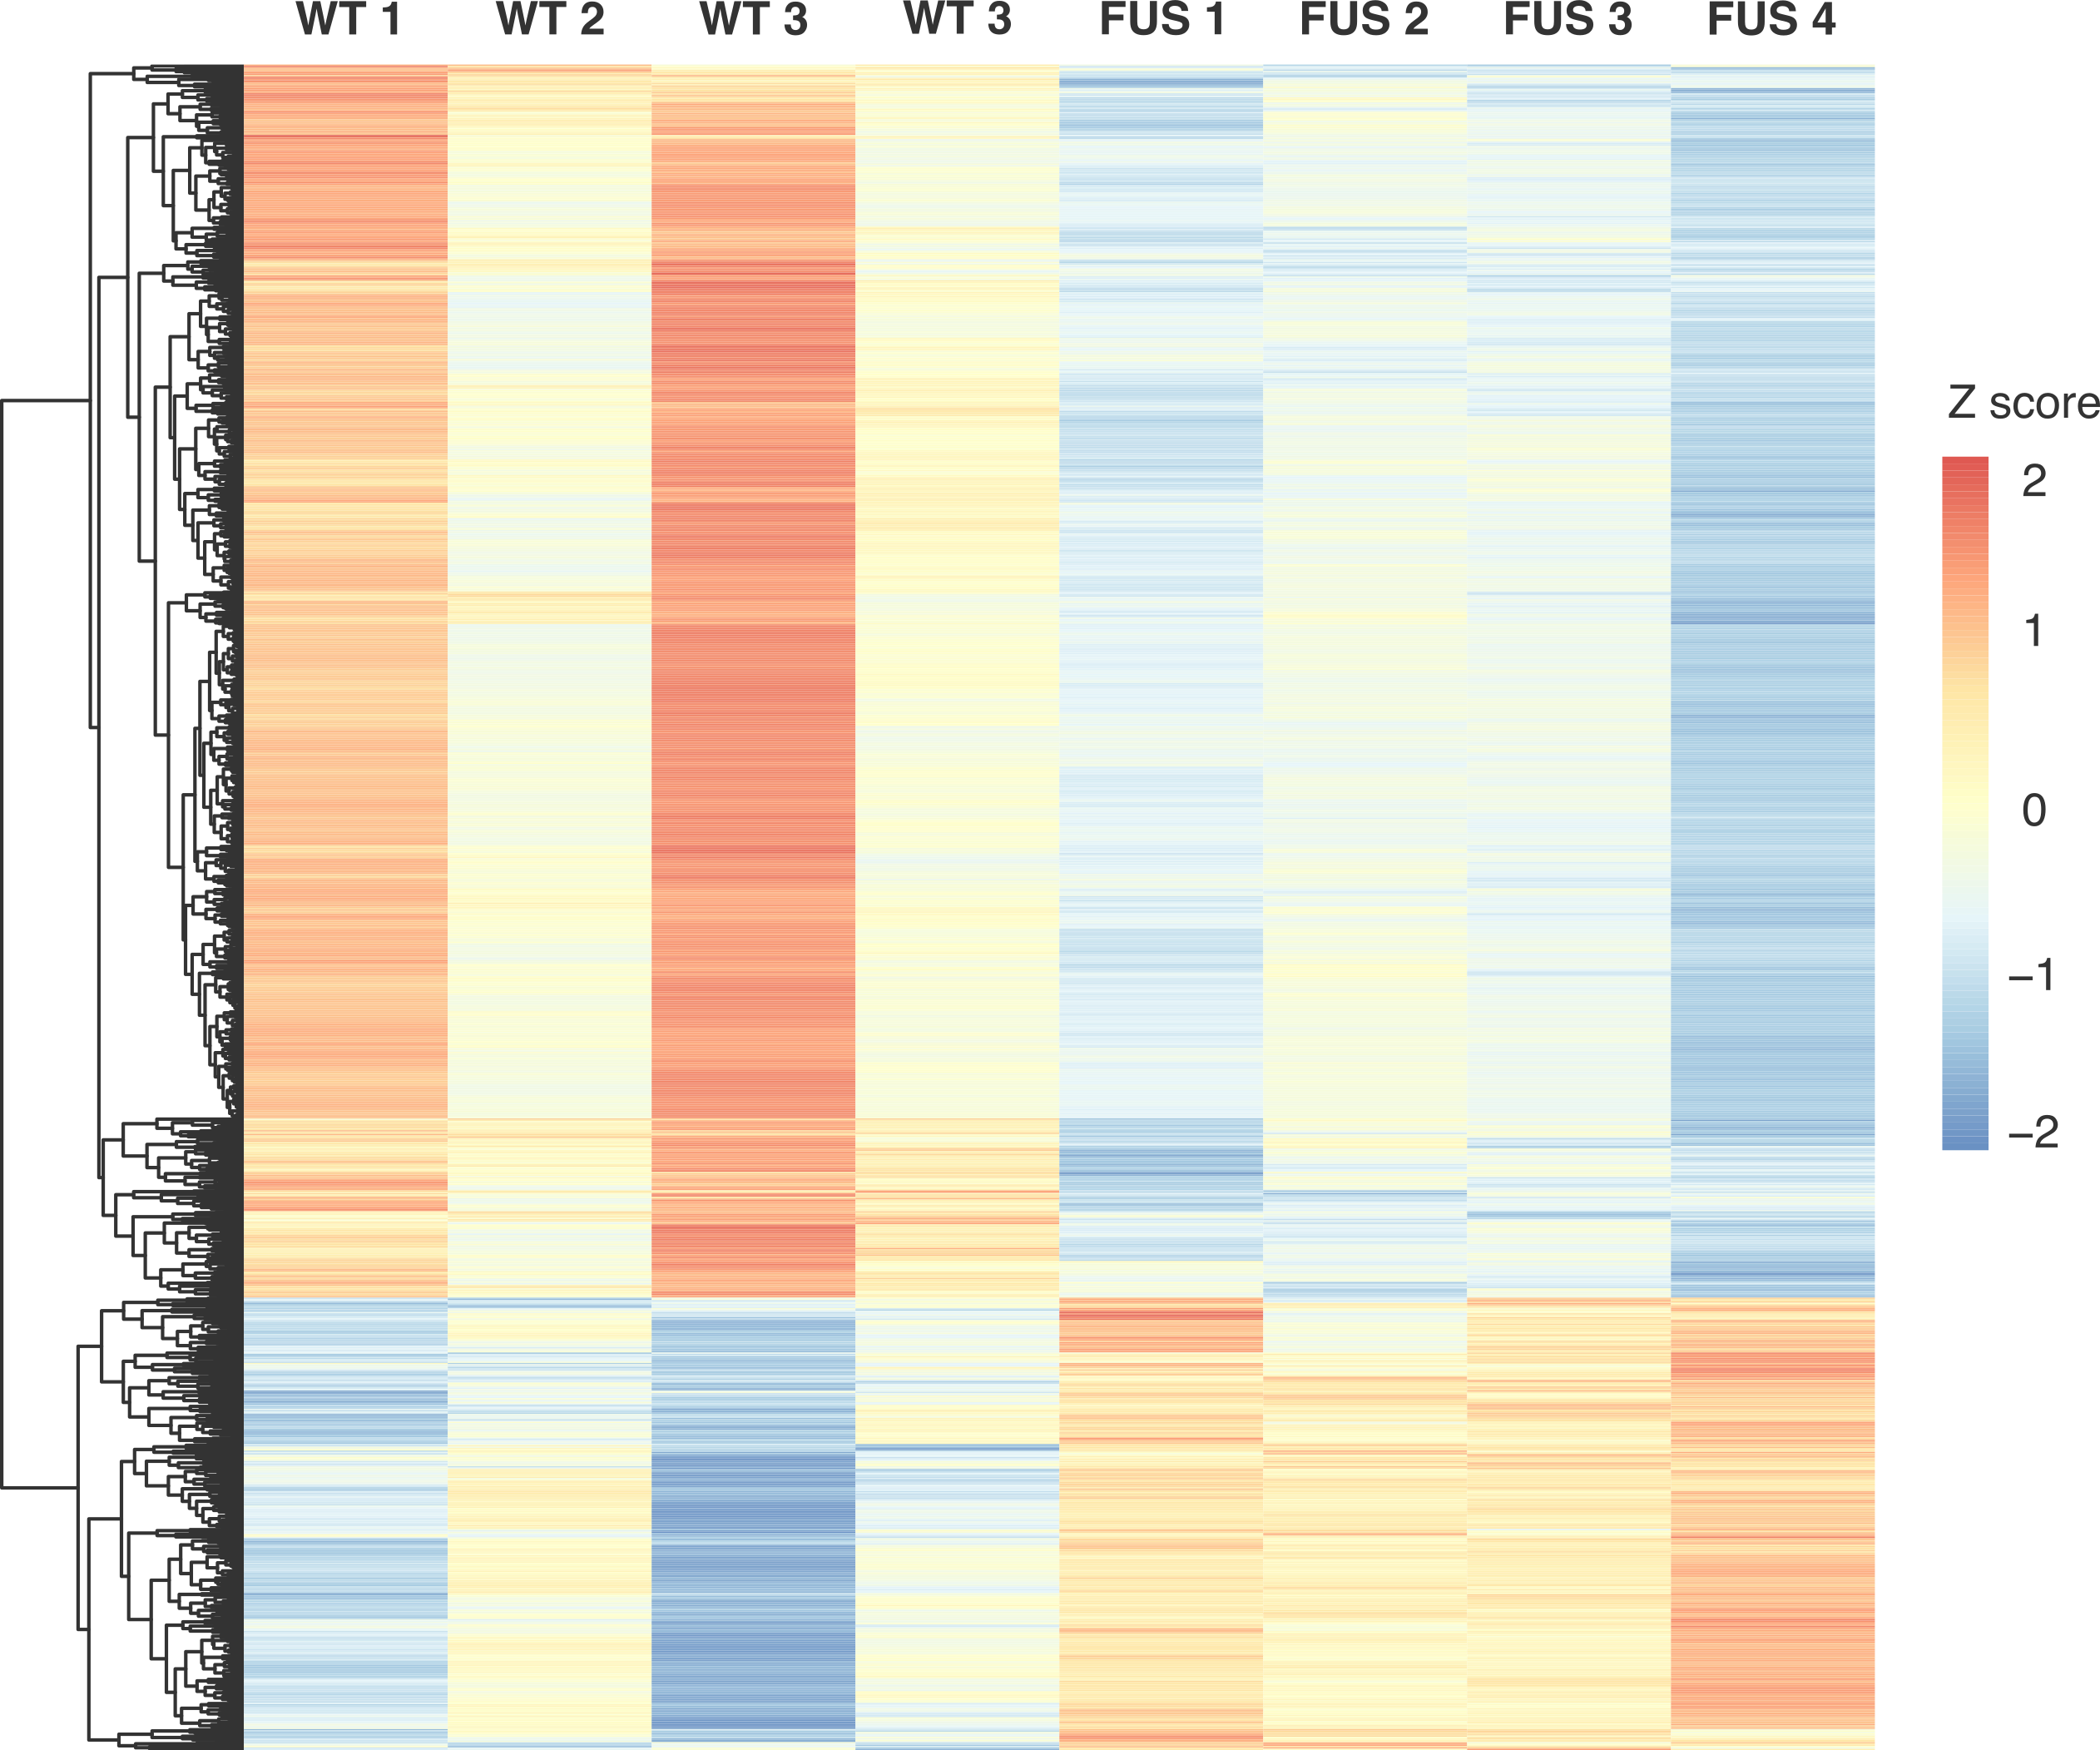
\includegraphics[width=\textwidth]{Figures/04_fus_mice/anny_normalised_heatmap.png}
	\caption[Z-score heatmap of the 12 month spinal cord dataset]{
		\textbf{Z-score heatmap of the 1289 differentially expressed genes in 12 month spinal cord dataset}
	WT: wildtype littermate; FUS: FUS $\Delta$14 heterozygote. 
}
	\label{fig:delta14_heatmap}
\end{figure}


\subsection{Gene ontology analysis indicates changes in mitochondrial and ribosomal pathways}
Genes from the 12 month spinal cord dataset differentially expressed at a relaxed threshold of \textit{P} < 0.005 were sent for gene ontology enrichment analysis. This compares the number of genes that are members of a particular ontology category with the expected distribution. This analysis identified a strong enrichment in genes belonging to mitochondria, ribosome and proteasome cateogories. Strikingly, almost all the genes in these categories were downregulated (Fig. \ref{fig:delta14_go}).

\begin{figure}[h!]
	\centering
	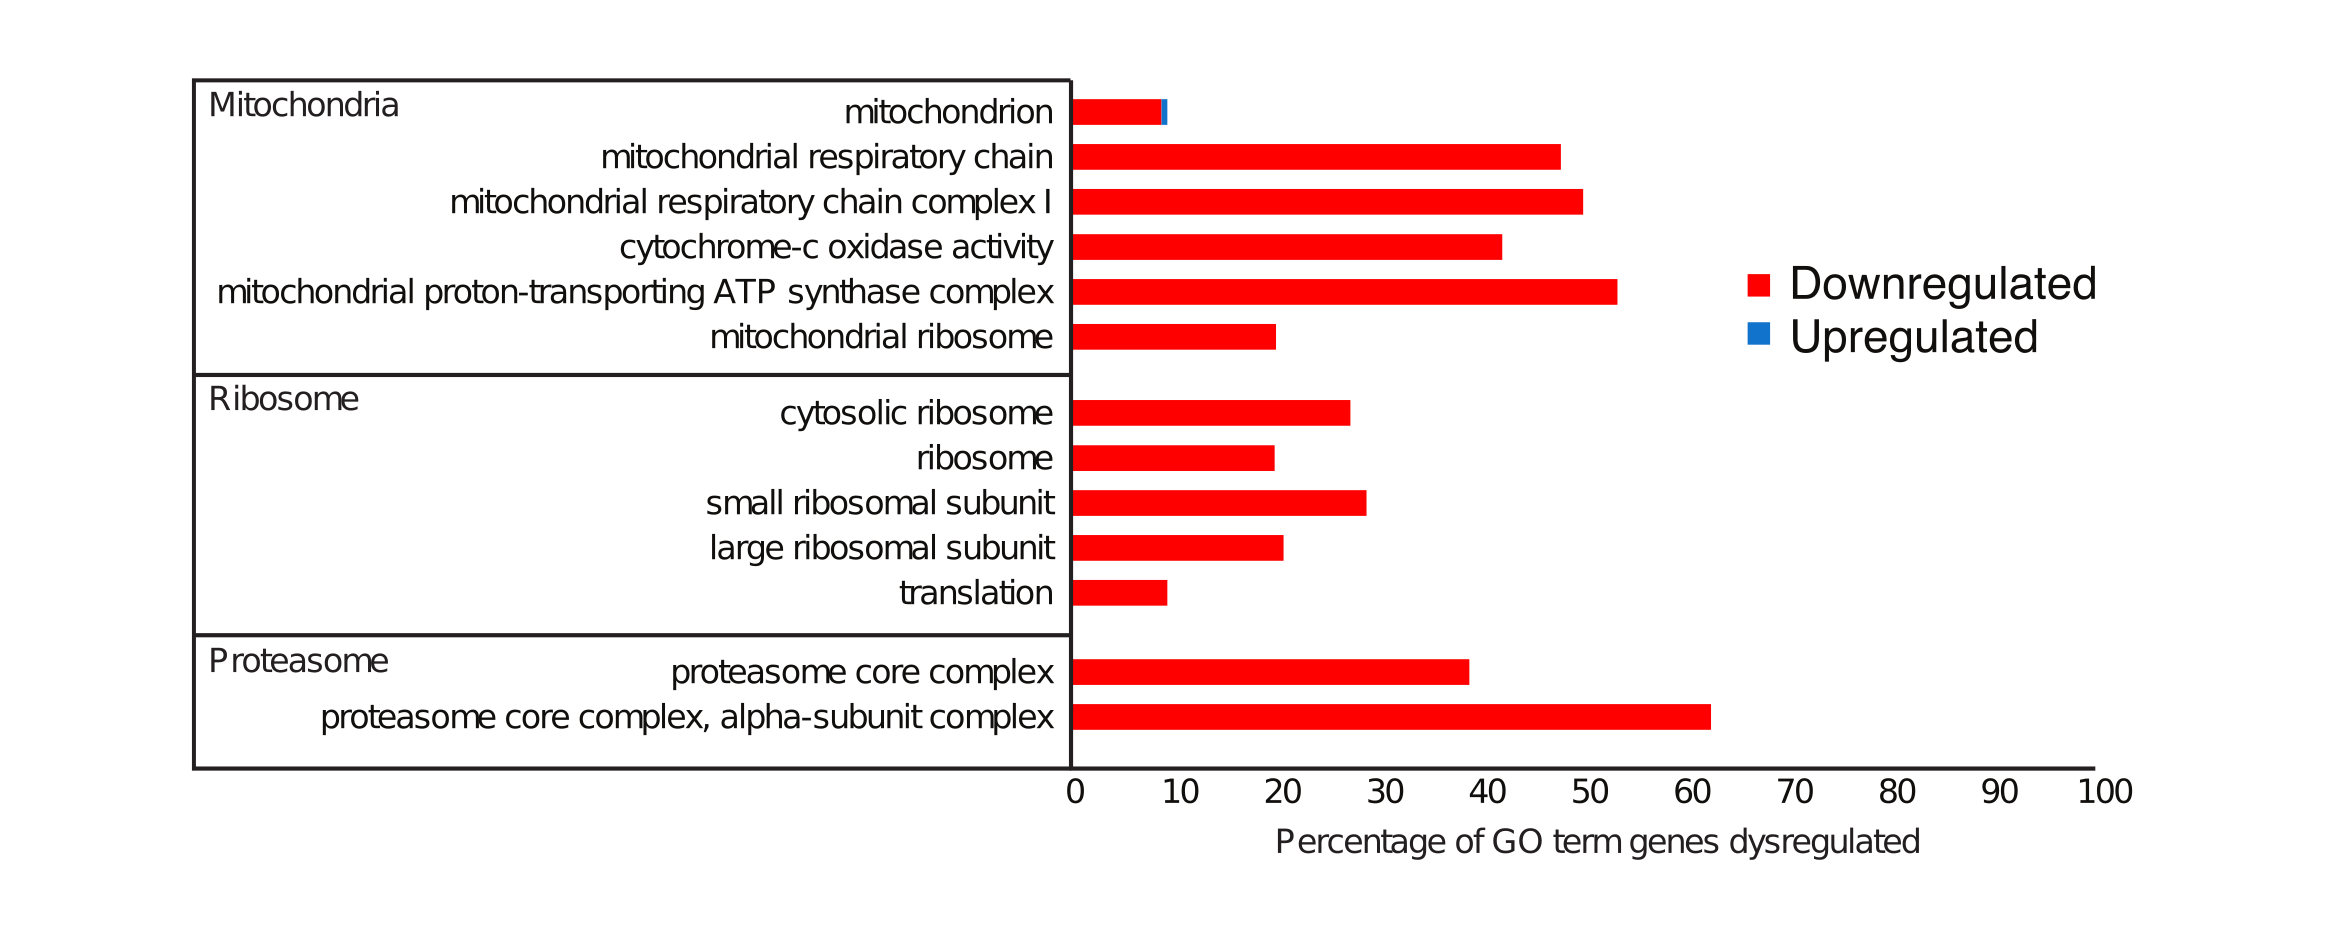
\includegraphics[width=\textwidth]{Figures/04_fus_mice/anny_GO_terms.png}
	\caption[Gene ontology categories in the 12 month spinal cord samples]{
		\textbf{Gene ontology categories significantly enriched in the 12 month FUS $\Delta$14 spinal cord samples}
		Each significant gene ontology category ( adjusted P < 0.05) is expressed as a proportion of upregulated (red) or downregulated (blue) genes.
	}
		\label{fig:delta14_go}
\end{figure}


\subsection{Splicing events are limited to FUS itself and few other genes}
Due to the lack of gene expression changes seen in other comparisons, differential splicing was assessed on 12 month spinal cord samples only.  
11 splicing events were found at FDR < 0.05, 4 of which were found in \textit{Fus} itself.
The top 2 splicing events in \textit{Fus} overlap exon 14, the skipping of which in the $\Delta$14 mice is classified as both an alternative last exon and an alternative start site.
The latter is a mis-annotation by \textit{SGSeq} due to the poor mappability of the central sequence of exon 14, leading to a gap in reads that span both ends of the exon.
The other 2 splicing events in \textit{Fus} are in the middle of the transcript where two introns, 6 and 7, are retained more in the wildtype mice and less retained in the $\Delta$14 mice.
Two overlapping complex events are seen in the \textit{Mbp} gene which encodes for Myelin basic protein, a major component of the myelin sheath. \textit{Mbp} is alternatively spliced to create different isoforms \citep{DeFerra1985}. A complex event involving 4 cassette exons is subtly altered in $\Delta$14.
\textit{Ewsr1} is a closely-related RNA-binding protein that interacts with FUS at the protein and RNA level \citep{Kapeli2016,Lagier-Tourenne2012}. 
A novel intron retention event in \textit{Ewsr1} is retained less in FUS $\Delta$14 mice.
This may in fact be a differential polyadenylation event that has previously been observed \citep{Rogelj2012} and mis-classified by the splicing software.
The other splicing events found affect 4 other genes of unknown significance.

\begin{table}[!htbp] 
	\centering 
	\caption[Splicing events found in 12 month spinal cord samples]{
		\textbf{Splicing events found in 12 month spinal cord samples}
	All splicing events found comparing FUS $\Delta$14 mice to wildtype at FDR < 0.05. 
	$log_2$FC: $log_2$ fold change.
	}
	\label{tab:fus_mouse_splicing} 
	\begin{tabular}{@{\extracolsep{5pt}} llccl} 
		\\[-1.8ex]\hline 
		\hline \\[-1.8ex] 
		Gene & type & $log_2$FC & FDR & coordinates (mm10)\\ 
		\hline \\[-1.8ex] 
		\textit{Fus} & alternate last exon & $-0.132$ & $1e^{-118}$ & chr7:127981291-127981458 \\ 
		\textit{Fus} & alternate start site & $-0.413$ & $1e^{-116}$ & chr7:127981522-127981791 \\ 
		\textit{Fus} & retained intron & $-0.217$ & $1e^{-13}$ & chr7:127974434-127975888 \\ 
		\textit{Fus} & retained intron & $-0.191$ & $1e^{-6}$ & chr7:127972770-127974400 \\ 
		\textit{Mbp} & complex  & $-0.014$ & $0.007$ & chr18:82575633-82584116 \\ 
		\textit{Mbp} & complex & $0.022$ & $0.007$ & chr18:82575633-82584112 \\ 
		 \textit{Ewsr1} & retained intron & $-0.066$ & $0.014$ & chr11:5079485-5078952 \\ 
		\textit{Cyhr1} & alternate 3\'\ splice site & 0.127 & $0.028$ & chr15:76659955-76659439 \\ 
		\textit{Gm32856} & alternate 3\'\ splice site & $-0.317$ & $0.038$ & chr8:129281397-129282476 \\ 
		\textit{Cd47} & cassette exon & 0.148 & $0.038$ & chr16:49906812-49910869 \\ 
		\textit{A330023F24Rik} & retained intron & 1.420 & $0.044$ & chr1:195021564-195021688 \\ 
		\hline \\[-1.8ex] 
	\end{tabular} 
\end{table} 

% 1 and 2 are due to delta 14 splicing
% mis-annotated as alternate start due to low mappability of exon 14


\section{Discussion}
My gene expression analysis demonstrates a progressive and tissue-specific change in RNA regulation, with 1,289 genes differentially expressed in the spinal cord of 12 month mutant mice. This finding is complemented by other contributions to the project. Behavioural experiments have shown the $\Delta$14 mice to have a progressive loss of motor function that is observable from 12 months of age. In addition, a reduction in number of motor neurons in the lumbar spinal cord has been observed from 12 months onwards, accompanied by an increase in cytoplasmic mislocalisation specifically of the mutant FUS.
The broad downregulation of mitochondrial, ribosomal and proteasomal genes specifically in the spinal cord of late-stage mice is an interesting finding that deserves further investigation. 
A recent study of a mouse model where mouse FUS was entirely replaced by either wildtype or ALS mutant human FUS showed similar downregulation of ribosomal (but not mitochondrial) genes \citep{Lopez-Erauskin2018}.
An enrichment of mitochondrial GO categories was previously seen in a FUS knockdown experiment conducted in human embryonic kidney cells  \citep{Schwartz2012}, suggesting that mitochondrial changes may be due to a loss of normal FUS function. Mitochondrial defects have been observed in the brains of FTD-FUS patients accompanied by FUS translocating to mitochondria \citep{Deng2015}. FUS overexpression has also been observed to cause mitochondrial defects at the neuromuscular junction \citep{So2018}. This points to an important role for FUS in mitochondria that may be perturbed by the $\Delta$14 mutation.
As mutant FUS has been shown to impair axonal transport \citep{Guo2017}, this impairment could explain the changes seen in both ribosomal and proteasomal transcripts.
% mitochondrial and ribosomal changes - new papers!

FUS knockout and knockdown experiments have demonstrated that large numbers of splicing events are sensitive to FUS protein levels \citep{Rogelj2012,Lagier-Tourenne2012,Ishigaki2012,Honda2014,Scekic-zahirovic2016}. The small number of splicing events found in the 12 month spinal cord samples suggest that the $\Delta$14 mutation has little affect on splicing with the exception of the \textit{Fus} transcript itself. The two \textit{Fus} intron retention events seen to be less retained in $\Delta$14 compared to wildtype as well as the events seen in \textit{Mbp} and \textit{Ewsr1} are deserving of further study. Defects in myelination have been seen in another FUS NLS mutation \citep{Scekic-zahirovic2017} and this may explain the changes seen in the myelin component \textit{Mbp}. The fellow FET family member \textit{Ewsr1} is also mis-spliced in FUS $\Delta$14. As it is also an intron retention event which changes in the same direction as those seen in \textit{Fus}, this could imply a connection between FUS and \textit{Ewsr1} at the RNA level.